\documentclass{article}

\usepackage{microtype}
\usepackage{graphicx}
\usepackage{subfigure}
\usepackage{booktabs}
\usepackage{hyperref}

\newcommand{\theHalgorithm}{\arabic{algorithm}}

% Use \usepackage{icml2025} for blind review.
\usepackage[accepted]{icml2025}

\usepackage{amsmath}
\usepackage{amssymb}
\usepackage{mathtools}
\usepackage{amsthm}

\usepackage[capitalize,noabbrev]{cleveref}

\theoremstyle{plain}
\newtheorem{theorem}{Theorem}[section]
\newtheorem{proposition}[theorem]{Proposition}
\newtheorem{lemma}[theorem]{Lemma}
\newtheorem{corollary}[theorem]{Corollary}
\theoremstyle{definition}
\newtheorem{definition}[theorem]{Definition}
\newtheorem{assumption}[theorem]{Assumption}
\theoremstyle{remark}
\newtheorem{remark}[theorem]{Remark}

\usepackage[textsize=tiny]{todonotes}

\icmltitlerunning{All skip-connections can be expanded indifinetly: Dynamical Representation on Vision Models}

\begin{document}

\twocolumn[
\icmltitle{All skip-connections can be expanded indifinetly: Dynamical Representation on Vision Models with Differential Geometry}

\begin{icmlauthorlist}
\icmlauthor{Jaume Ivars Grimalt}{comp}
\end{icmlauthorlist}

\icmlaffiliation{comp}{Mycrospace AI Research, Valencia, Spain}

\icmlkeywords{Machine Learning, ICML}

\vskip 0.3in
]

\printAffiliationsAndNotice{}

\begin{abstract}
Residual networks are often read as forward Euler discretizations of an ordinary differential equation (ODE),
yet trained ResNets need not converge to a smooth ODE as depth grows.
We study what happens when every residual block $x + f_k(x)$ of a pretrained vision model is replaced
by $N$ Euler steps of size $1/N$ on the same block.
On ResNet-50, ResNet-101, Swin, ConvNeXt and a weight-tied ConvNeXt trained by us,
top-1 accuracy on ImageNet drops by less than 2 points even for $N=10{,}000$,
and fine-tuning only the last stage and the classification head recovers almost all of the gap.
In ConvNeXt, repeating the blocks with unit steps instead collapses accuracy to chance level.
We explain this behaviour by describing a residual network as a composition of ODE solvers:
an accurate Euler discretization of a switched ODE that is autonomous inside each block and discontinuous between blocks.
Building on this view, we propose methods to analyze feature trajectories at arbitrary depth resolution
without retraining, and use them to contrast the sawtooth dynamics of standard networks
with the smooth dynamics of weight-tied ones.
% Para la revision ciega: sustituir por un enlace anonimo (p. ej. anonymous.4open.science)
Code is available at \url{https://github.com/jaume2000/dynamics_skip_nn}.
\end{abstract}
%Therefore, we propose a method to exploit each parameter's significance across all network's computations. % Comment for now

\section{Introduction}
\label{sec:intro}

Residual connections \citep{he2016resnet} are part of almost every modern architecture,
from convolutional networks \citep{liu2022convnext} to vision transformers \citep{liu2021swin}.
They were introduced to solve the degradation problem, in which deeper plain networks reach a higher training error
than shallower ones.
\citet{he2016resnet} argue that this problem is not caused by vanishing gradients
\citep{vanishingGradient, glorot2010understanding}, which normalized initialization and batch normalization
\citep{ioffe2015batchnorm} already mitigate, and later work showed that residual connections also make the loss landscape
much smoother than in plain networks such as VGG
\citep{li2018visualizinglosslandscapeneural, simonyan2015deepconvolutionalnetworkslargescale}.

Beyond optimization, the most influential way of understanding what residual networks compute
is the dynamical systems view.
A residual block $x_{k+1} = x_k + f_k(x_k)$, where $x_k$ is the feature map entering block $k$
and $f_k$ is its residual branch, can be read as one forward Euler step of size $1$
of an ordinary differential equation (ODE) \citep{e2017proposal, haber2017stable, lu2018beyond}.
This view has inspired stable architectures \citep{haber2017stable},
reinterpretations of regularizers such as stochastic depth \citep{huang2016stochastic, lu2018beyond}
and continuous-depth models such as Neural ODEs \citep{chen2019neuralordinarydifferentialequations},
which still do not match the accuracy of standard discrete networks \citep{sander2022residualneuralnetworksdiscretize}.

Whether trained networks actually behave like ODE discretizations is far from settled.
\citet{sander2022residualneuralnetworksdiscretize} show that the distance between a ResNet
and its associated Neural ODE does not vanish with depth unless the residual functions are smooth in depth,
and \citet{cohen2021scaling} find that trained weights follow scaling regimes in which the Neural ODE limit
is not an adequate description.
\citet{queiruga2020continuousindepthneuralnetworks} argue that ResNets fail to behave as meaningful numerical integrators
and design ContinuousNets, which can be evaluated with different step sizes and integration schemes.
Two other readings compete with the dynamical one: residual networks as ensembles of shallow paths,
which explains why removing individual blocks at test time barely affects performance and reordering them
degrades it smoothly \citep{veit2016residualnetworksbehavelike}, and blocks as iterative refinement
of a shared representation \citep{greff2017highway, jastrzebski2018iterative}.
A similar robustness to skipping and reordering has been observed in the middle layers of large transformers
\citep{sun2025painters}.
It is still unclear in what sense, if any, a trained residual network is an ODE.

\begin{figure*}[t]
\centering
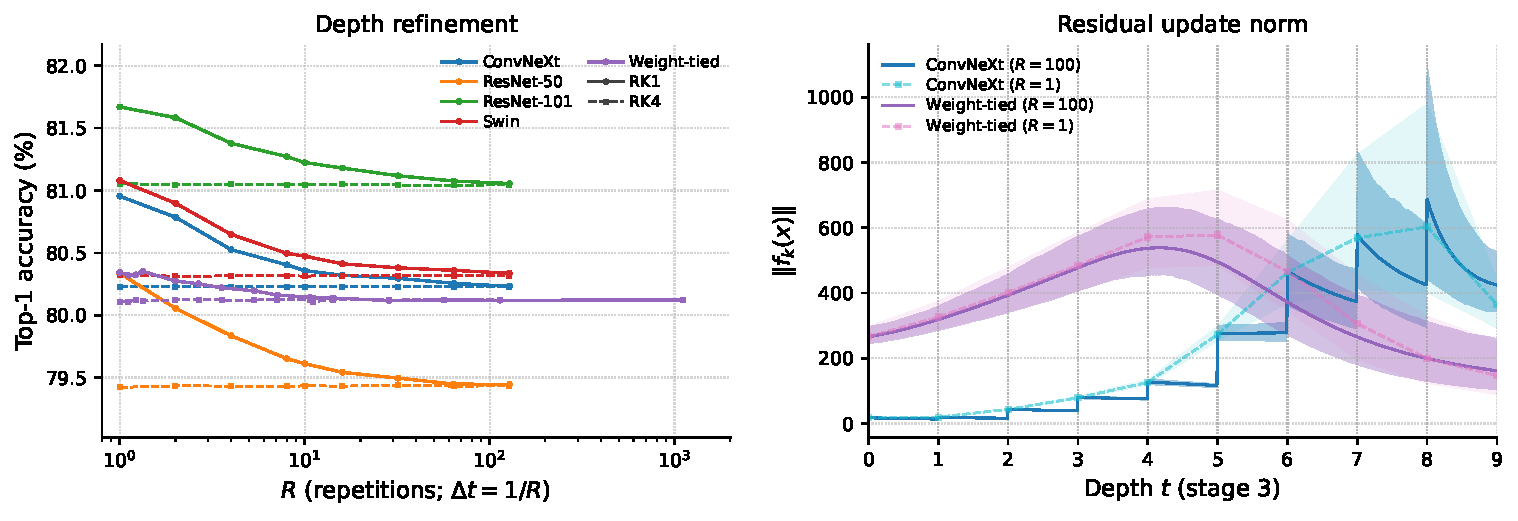
\includegraphics[width=\textwidth]{figures/teaser.pdf}
\caption{\textbf{Left:} top-1 accuracy on ImageNet-1k when every residual block of a pretrained model
is replaced by $N$ Euler steps of size $1/N$, with RK1 (solid, circles) and RK4 (dashed, squares).
For the weight-tied ConvNeXt, $N{=}1$ is the trained depth $D{=}9$ ($N{=}D/9$).
\textbf{Right:} mean residual-update norm $\|f_k(x)\|$ along depth over 500 images
(shaded: 5th–95th percentile across images), with a sawtooth profile in a standard ConvNeXt
and a smooth one when stage 3 shares a single block.}
\label{fig:teaser}
\end{figure*}

We start from a simple observation (\cref{fig:teaser}).
Take a pretrained vision model and replace every residual block by $N$ Euler steps of size $1/N$ on the same block,
$x \leftarrow x + \frac{1}{N} f_k(x)$ repeated $N$ times, with no fine-tuning.
On ResNet-50, ResNet-101 \citep{he2016resnet}, Swin \citep{liu2021swin} and ConvNeXt \citep{liu2022convnext},
top-1 accuracy on ImageNet-1k \citep{deng2009imagenet} drops by less than 2 points even with $N=10{,}000$,
and fine-tuning only the last stage and the classification head recovers almost all of the gap.
Repeating the blocks with unit steps instead collapses ConvNeXt to chance level with only ten repetitions,
so the residual functions are far from the identity.
Yet interpolating the weights of two consecutive blocks to build an intermediate one costs around 20 points.
Closest to our setting, \citet{chang2018multilevel} grow ResNets during training by splitting blocks
and halving the step size.
Here we apply the refinement to pretrained models, with no training at all.

These three facts are hard to reconcile with a single ODE whose parameters vary smoothly with depth,
but they follow naturally if we read the network as a composition of ODE solvers.
Within a stage, we describe a residual network as the forward Euler discretization of a switched ODE
\citep{liberzon2003switching},
\begin{equation}
\frac{dx}{dt} = f\big(x;\theta(t)\big), \qquad \theta(t) = \theta_k \ \text{ for } t \in [k, k+1),
\label{eq:switched}
\end{equation}
where $\theta_k$ are the parameters of block $k$.
Inside each block the system is autonomous, and a single Euler step of size $1$ is already an accurate approximation
of the flow of $f(\cdot;\theta_k)$ over one unit of time, which is why refining it changes almost nothing.
Between blocks the vector field switches abruptly, which is why there is no smooth $\theta(t)$ to interpolate.
Under this reading, the dynamical systems view and the results of \citet{sander2022residualneuralnetworksdiscretize}
and \citet{cohen2021scaling} are compatible: a trained ResNet is not a discretization of a smooth Neural ODE,
but it is an accurate discretization of a piecewise autonomous one.

This model raises a natural question: how different do the vector fields of consecutive blocks need to be?
Weight-tied residual networks \citep{liao2016bridging, sharesnet}, looped transformers
\citep{dehghani2019universal, giannou2023looped} and deep equilibrium models \citep{bai2019deep}
show that a single block applied repeatedly can do much of the work of a stack of distinct ones.
We test the extreme case in which all blocks of a stage share their weights,
which turns the stage into a single autonomous ODE.
A ConvNeXt-T whose stage 3 shares one block loses only 0.6 points of top-1 accuracy
while removing 10M of its 28M parameters.
Its accuracy stays within 0.2 points when the stage is integrated over the same time horizon with up to 10,000 steps,
and Euler, second order Runge-Kutta (RK2) and fourth order Runge-Kutta (RK4) integrators converge to the same accuracy.

Finally, depth refinement lets us sample the trajectory of the features at arbitrary resolution without retraining.
We use it to study the geometry of these trajectories, in particular their speed and the change of direction
between consecutive steps.
Standard ResNet and ConvNeXt models show a sawtooth velocity profile, where speed jumps at every block switch
and decays inside the block, while weight-tied networks show a smooth one.
% TODO: ampliar a Swin y ResNet-101 cuando esten los resultados

Our contributions are:
\begin{itemize}
    \item We show that a weight-tied stage, a single autonomous ODE, recovers most of the accuracy
    of a standard ConvNeXt with 10M fewer parameters, and is insensitive to the integrator and the number of steps
    (\cref{sec:sharing}).
    \item We propose methods to analyze feature trajectories in depth, and use them to characterize the smooth
    dynamics of weight-tied networks (\cref{sec:geometry-tied}).
    \item We show that per-block depth refinement with step $1/N$ preserves the accuracy of pretrained ResNet,
    Swin and ConvNeXt models without fine-tuning, while unit-step repetition and weight interpolation between blocks fail,
    and we explain this with the switched ODE model of \cref{eq:switched} (\cref{sec:refinement}).
    % TODO: si mides el error de un paso de Euler frente al flujo de cada bloque, anadirlo aqui
    \item We contrast the switched dynamics of standard networks with the smooth dynamics of weight-tied ones
    using the refined trajectories (\cref{sec:geometry-continuized}).
\end{itemize}

\section{Sharing parameters}
\label{sec:sharing}
% Talk about convnext, our own convnext: all stages sahred, shared Stage 3, fine-tune over stage 4 after expanding the network.
% Then, talk about network expansion and ablations on this: Euer, RK4, different N...
% Point out the result of the experiment with a sentence

\section{Differential Geometry applied to Weight-tied Neural Network Representational Dynamics}
\label{sec:geometry-tied}
% Talk about the metrics you used and its interpretation (cosine distance, feature map cosine distance, curvature...)
% Show the phase plane, ...
% Results on D=9 vs D=100

\section{Infinite-resolution without fine-tunning}
\label{sec:refinement}

\section{Differential Geometry of continuized residual networks}
\label{sec:geometry-continuized}

\bibliography{paper}
\bibliographystyle{icml2025}

\end{document}